\documentclass[a4paper, 12pt]{article}
\usepackage{../../Templates/package}
\usepackage{amssymb}
\usepackage{graphicx}
\usepackage[export]{adjustbox}
\usepackage{framed}
\graphicspath{{../../Assets}}

\newcommand{\Titolo}{Manuale Utente}
\newcommand{\Data}{19/05/2024}
\newcommand{\Versione}{1.0.0}
\newcommand{\Descrizione}{Questo documento fornisce istruzioni dettagliate sull'utilizzo della \textit{web app} EasyMeal.}
\newcommand{\Verificatori}{
    Alessandro Tigani Sava, \\
    & Davide Maffei, \\
    & Niccolò Carlesso, Carlo Rosso     
}
\newcommand{\Redattori}{ 
     Matteo Bando, \\
    & Giacomo Gualato, Davide Maffei, \\
    &  Carlo Rosso     
}
\newcommand{\Approvatori}{Davide Maffei}
\newcommand{\Destinatari}{
    Prof.\ Tullio Vardanega \\ 
    & Prof.\ Riccardo Cardin \\ 
    & Alessandro Staffolani
}
\newcommand{\Stato}{Approvato}

\newcommand{\Gruppo}{SWEnergy}
\newcommand{\Mail}{\href{mailto:project.swenergy@gmail.com}{project.swenergy@gmail.com}}

\renewcommand\familydefault{\sfdefault} % Set default font family to sans-serif
\linespread{1.5}

\hypersetup{
	pdfmenubar=true,            % show Acrobat’s menu?
	pdfstartview={FitH},        % fits the width of the page to the window
	colorlinks=true,            % false: boxed links; true: colored links
	linkcolor=black,            % color of internal links (change box color with linkbordercolor)
	% citecolor=green,          % color of links to bibliography
	% filecolor=magenta,        % color of file links
	urlcolor=[RGB]{156,1,198}   % color of external links
}

\newcommand{\copertina}{
	\begin{titlepage}
		\vspace*{-3.5cm}
		\makebox[\textwidth]{
\includegraphics[width=\paperwidth]{header.png}}
		\begin{center}
			
\includegraphics[width=1\textwidth]{logo.png}	\\
			\vspace{1cm}
			\Mail	\\
			\vspace{0.5cm}
			\textbf{\begin{LARGE} \Titolo \end{LARGE}}		\\
			\vspace{1cm}
			\textbf{Descrizione:} \Descrizione{}			\\
			\vspace{1cm}
			\begin{tabular}{ll}
				\textbf{Stato}               & \Stato              \\
				\textbf{Data}                & \Data               \\
				\midrule
				\textbf{Redattori}           & \Redattori          \\
				\textbf{Verificatori}        & \Verificatori       \\

				\ifdefined\Approvatori
				\textbf{Approvatori}         & \Approvatori        \\
				\fi

				\ifdefined\ApprovatoriInterni
				\textbf{Approvatori interni} & \ApprovatoriInterni \\
				\fi

				\ifdefined\ApprovatoriEsterni
				\textbf{Approvatori esterni} & \ApprovatoriEsterni \\
				\fi

				\ifdefined\Destinatari
				\textbf{Destinatari}         & \Destinatari        \\
				\fi

				\midrule

				\ifdefined\Versione
				\textbf{Versione}            & \Versione           \\
				\fi
			\end{tabular}
		\end{center}
		\vspace{4cm}
	\end{titlepage}
	\newpage
}

\fancypagestyle{plain}{
	\fancyhf{}
	\rhead{ 
\includegraphics[scale=0.05]{horizontal_logo.png}}
	\lhead{\Titolo \ifdefined\Versione \ \Versione \fi}
	%\lfoot{\Titolo}
	\rfoot{\thepage{} di \pageref{LastPage}}
	\renewcommand{\headrulewidth}{0.2pt}
	\renewcommand{\footrulewidth}{0.2pt}
}
\pagestyle{plain}


\begin{document}
\copertina{}
\section*{Registro delle modifiche}
 {
  \scriptsize
  \begin{tabular}{p{0.10\linewidth}p{0.10\linewidth}p{0.15\linewidth}p{0.15\linewidth}p{0.15\linewidth}p{0.19\linewidth}}
	  \textbf{Versione} & \textbf{Data} & \textbf{Redattore}     & \textbf{Verificatore} & \textbf{Approvatore} & \textbf{Descrizione}                                                                                                                     \\
	  \toprule
	  2.0.1             & 27/02/2024    & Davide Maffei          & Carlo Rosso           & /                    & Correzioni in seguito alla revisione RTB                                                                                                 \\
	  \hline
	  2.0.0             & 27/02/2024    & /                      & /                     & Niccolò Carlesso     & Approvazione finale del documento                                                                                                        \\
	  \hline
	  1.5.0             & 26/02/2024    & Alessandro Tigani Sava & Carlo Rosso           & /                    & Descrizione metriche di qualità                                                                                                          \\
	  \hline
	  1.4.1             & 14/02/2024    & Davide Maffei          & Giacomo Gualato       & /                    & Allineamento delle sezioni dei ruoli                                                                                                     \\
	  \hline
	  1.4.0             & 14/02/2024    & Davide Maffei          & Giacomo Gualato       & /                    & Creazione delle sezioni dei processi primari, di supporto e organizzativi                                                                \\
	  \hline
	  1.3.0             & 8/01/2024     & Carlo Rosso            & Niccolò Carlesso      & /                    & Correzione della sotto-sezione "Aggiornamento delle "Norme di Progetto"" e aggiunte le sotto-sezioni "Revisione del codice" e "Codifica" \\
	  \hline
	  1.2.0             & 31/12/2023    & Carlo Rosso            & Niccolò Carlesso      & /                    & Ristrutturazione del documento per ruolo, piuttosto che per argomento                                                                    \\
	  \hline
	  1.1.0             & 30/10/2023    & Carlo Rosso            & Giacomo Gualato       & /                    & Aggiornamento della sezione dedicata alla documentazione e aggiunta una sezione dedicata agli appunti                                    \\
	  \hline
	  1.0.0             & 30/10/2023    & /                      & /                     & Giacomo Gualato      & Approvazione finale del documento                                                                                                        \\
	  \hline
	  0.2.1             & 29/10/2023    & Alessandro Tigani Sava & Niccolò Carlesso      & /                    & Modifica procedure in sezione Approvazione di un documento                                                                               \\
	  \hline
	  0.2.0             & 24/10/2023    & Matteo Bando           & Niccolò Carlesso      & /                    & Redazione sezioni Versionamento, Verifica di un documento, Approvazione di un documento                                                  \\
	  \hline
	  0.1.0             & 23/10/2023    & Alessandro Tigani Sava & Matteo Bando          & /                    & Redazione sezioni Introduzione, Strumenti, Creazione e modifica di un documento, Ruoli, Registro delle modifiche                         \\
	  \hline
  \end{tabular}
 }

\newpage

\setcounter{tocdepth}{3}
\tableofcontents
\newpage
\section{Introduzione}

Il presente documento, intitolato "Piano di Progetto", descrive e spiegare le
decisioni organizzative adottate dal gruppo SWEnergy per lo sviluppo del
progetto "\textit{Easy Meal}", proposto dall'azienda
\href{https://imolainformatica.it/}{Imola Informatica}. Il "Piano di Progetto" è
suddiviso nelle seguenti sezioni:

\begin{itemize}
	\item \textbf{Analisi dei rischi}: identifica i rischi individuati dal
	      gruppo e le strategie per mitigarli;

	\item \textbf{Modello di sviluppo}: descrive l'organizzazione temporale del
	      team di SWEnergy;

	\item \textbf{Pianificazione}: dettaglia la pianificazione del lavoro del
	      gruppo, incluse le attività, le risorse e i tempi necessari per lo
	      sviluppo del progetto;

	\item \textbf{Preventivo}: presenta il preventivo delle ore di lavoro e il
	      costo totale del progetto;

	\item \textbf{Consuntivo}: riporta le ore di lavoro e il costo effettivo del
	      progetto fino al momento della stesura del piano di progetto della
	      fase corrente: RTB.
\end{itemize}

\subsection{Scopo del documento}

Questo documento ha lo scopo di raccogliere in modo organico, coerente e
uniforme tutte le informazioni riguardanti la pianificazione del progetto, al
fine di fornire un riferimento per la gestione dello stesso. Al termine della
prima fase del progetto (RTB), verrà utilizzato per valutare l'andamento del
lavoro e per spiegare le decisioni adottate durante la pianificazione.

\subsection{Scopo del prodotto}

"\textit{Easy Meal}" è una web app progettata per gestire le prenotazioni
presso i ristoranti, sia dal lato dei clienti che dei ristoratori. Il prodotto
finale sarà composto da due parti:

\begin{itemize}
	\item \textbf{Cliente}: consente ai clienti di prenotare un tavolo presso un
	      ristorante, visualizzare il menù e effettuare un ordine;

	\item \textbf{Ristoratore}: consente ai ristoratori di gestire le
	      prenotazioni e gli ordini dei clienti, oltre a visualizzare la lista
	      degli ingredienti necessari per preparare i piatti ordinati.
\end{itemize}

\subsection{Glossario}

Al fine di evitare ambiguità linguistiche e garantire un'utilizzazione coerente
delle terminologie nei documenti, il gruppo ha redatto un documento interno
chiamato "Glossario". Questo documento definisce in modo chiaro e preciso i
termini che potrebbero generare ambiguità o incomprensione nel testo. I termini
presenti nel Glossario sono identificati da una 'G' (per esempio parola$_G$) a
pedice.

\subsection{Riferimenti}

\subsubsection{Normativi}
\begin{itemize}
	\item "\textit{Way of Working}";
	\item 	\href{https://www.math.unipd.it/~tullio/IS-1/2023/Progetto/C3.pdf}
	      {Documento del capitolato d'appalto C3 - \textit{Easy Meal}};
	\item \href{https://www.math.unipd.it/~tullio/IS-1/2023/Dispense/PD2.pdf}
	      {Regolamento del progetto};
\end{itemize}

\subsubsection{Informativi}

Slide dell'insegnamento di Ingegneria del Software:
\begin{itemize}
	\item \href{https://www.math.unipd.it/~tullio/IS-1/2023/Dispense/T3.pdf}
	      {Modelli di sviluppo del software};
	\item \href{https://www.math.unipd.it/~tullio/IS-1/2023/Dispense/T4.pdf}
	      {Gestione di progetto};
	\item \href{https://www.math.unipd.it/~tullio/IS-1/2023/Dispense/T5.pdf}
	      {Analisi dei requisiti};
\end{itemize}

\subsection{Scadenze}
Il \textit{team} di SWEnergy si impegna a rispettare le seguenti scadenze per il
completamento del progetto:
\begin{itemize}
	\item \textbf{Prima revisione (avanzamento RTB}: 21 dicembre 2023;
	\item \textbf{Seconda revisione (avanzamento PB)}: da definire;
	\item \textbf{Terza revisione (avanzamento CA)}: da definire;
\end{itemize}

\newpage

\section{Requisiti}
Questa sezione fornisce un elenco dei requisiti minimi indispensabili per l'esecuzione dell'applicazione, illustrando le caratteristiche necessarie per configurare 
correttamente l'ambiente di sviluppo del progetto.

\subsection{Requisiti di sistema}
Affinché l'installazione e l'avvio del prodotto avvengano senza problemi e per garantire un'esperienza completa e soddisfacente nell'utilizzo 
dell'applicazione, è essenziale installare i seguenti \textit{software}.

\begin{longtable}{|c|c|c|}
	\hline
	\textbf{Componente}       & \textbf{ Versione}   & \textbf{ Riferimenti per il download} \\
	\hline
     Node.js             & $ \geq  20.x.x$            &\href{https://nodejs.org/en/}{https://nodejs.org/en/}        \\
    \hline
     npm                & $ \geq 9.x.x$            &Integrato con il download di Node.js        \\
    \hline

    \caption{Tabella dei requisiti di sistema.}
\end{longtable}


\subsection{Requisiti \textit{software}}
L'applicazione è stata testata e confermata come utilizzabile sui principali \textit{browser}, per i quali sono specificate le versioni iniziali che hanno costituito 
il punto di partenza per lo sviluppo del progetto. Durante lo sviluppo, si è considerato incrementalmente l'aggiornamento alle versioni più recenti dei singoli \textit{browser}.

\begin{longtable}{|c|c|c|}
	\hline
	\textbf{Browser}       & \textbf{ Versione}    \\
	\hline
    Google Chrome             & 123                    \\
    \hline
    Arc                       & 1.26                    \\
    \hline
    Opera GX                       & 124                    \\
    \hline
    Safari                        & 17.3                    \\
    \hline
    Microsfot Edge                 & 123                      \\
    \hline

    \caption{Tabella dei requisiti \textit{software}.}
\end{longtable}


\subsection{Requisiti \textit{hardware}}
Poiché l'applicazione funziona su un \textit{browser}, non ci sono requisiti specifici definiti dal proponente, dal capitolato o dal progetto stesso. 
Quindi, i seguenti requisiti sono considerati solo come linee guida generali per l'esecuzione del prodotto creato.

\begin{longtable}{|l|p{0.8\textwidth}|}
	\hline
	\textbf{Componente}       & \textbf{ Requisito minimo}   \\
	\hline
     Processore             &  Processore a 64 bit Quad-Core 3,2 GHz      \\
    \hline
     Memoria RAM            &  4GB DDR4       \\
    \hline
    Spazio su disco         & $ \geq  126 GB$         \\
    \hline
    Connessione Internet         & Connessione \textit{Internet} stabile e veloce, in grado di supportare le esigenze di traffico dell'applicazione         \\
    \hline

    \caption{Tabella dei requisiti \textit{hardware}.}
\end{longtable}
\section{Utente non autenticato}
Come utente non autenticato, hai accesso a una serie di funzionalità di base che 
ti permettono di esplorare EasyMeal e di accedere o registrarti.

\subsection{Header}

\begin{figure}[htbp]
    \centering
	
\includegraphics[width=0.8\textwidth]{PB/manuale-utente/header-non-autenticato.png}
    \caption{Barra di Navigazione per l'utente non autenticato}
\end{figure}

La barra di navigazione in alto ti permette di accedere facilmente alle varie 
sezioni della piattaforma. 
Puoi tornare alla schermata principale cliccando sul logo EasyMeal o sul nome 
EasyMeal entrambi posti in alto a sinistra. Allo stesso modo si può cliccare su
\texttt{Esplora} per effettuare la medesima operazione. Infine, si può cliccare
su \texttt{Login} per accedere alla schermata di login e su 
\texttt{Registrati} per accedere alla schermata di registrazione.

\subsection{Footer}

\begin{figure}[htbp]
    \centering
	
\includegraphics[width=0.8\textwidth]{PB/manuale-utente/footer.png}
    \caption{Footer}
\end{figure}

Il footer si trova in fondo ad ogni pagina. In viola sono evidenziati i link
cliccabili che ti permettono di accedere alle sezioni di EasyMeal. In
particolare, da sinistra verso destra, dall'alto verso il basso si ha:
\begin{itemize}
	\item \textbf{\texttt{Project SWEnergy Website}}: questo collegamento permette di
		accedere al sito web del gruppo SWEnergy, che ha sviluppato EasyMeal.
		In particolare, il sito contiene informazioni sul gruppo e i documenti
		del progetto EasyMeal;

	\item \textbf{Navigazione}: sotto questa voce sono presenti i link "About
		us" e "Esplora". Il primo link è collegato ad una pagina che introduce
		il progetto EasyMeal. Il secondo riporta alla pagina di esplorazione dei
		ristoranti;

	\item \textbf{\texttt{Autenticazione}}: questa voce rimanda ad una pagina di
		selezione della tipologia di login e di registrazione. In particolare,
		si tratta di una pagina dedicata alle quattro voci sotto di essa. Sotto
		questa voce sono presenti i link \texttt{Login clienti}, 
		\texttt{Registrazione clienti}, \texttt{Login ristoratori} e 
		\texttt{Registrazione ristoratori}. Questi
		link permettono di accedere alle pagine di login e registrazione per
		clienti e ristoratori;

	\item \textbf{Contatti}: viene mostrata la mail di contatto del gruppo
		SWEnergy, per permettere agli utenti di contattare il gruppo per
		eventuali problemi o domande;
\end{itemize}


\subsection{Home Page}

\begin{figure}[htbp]
    \centering
	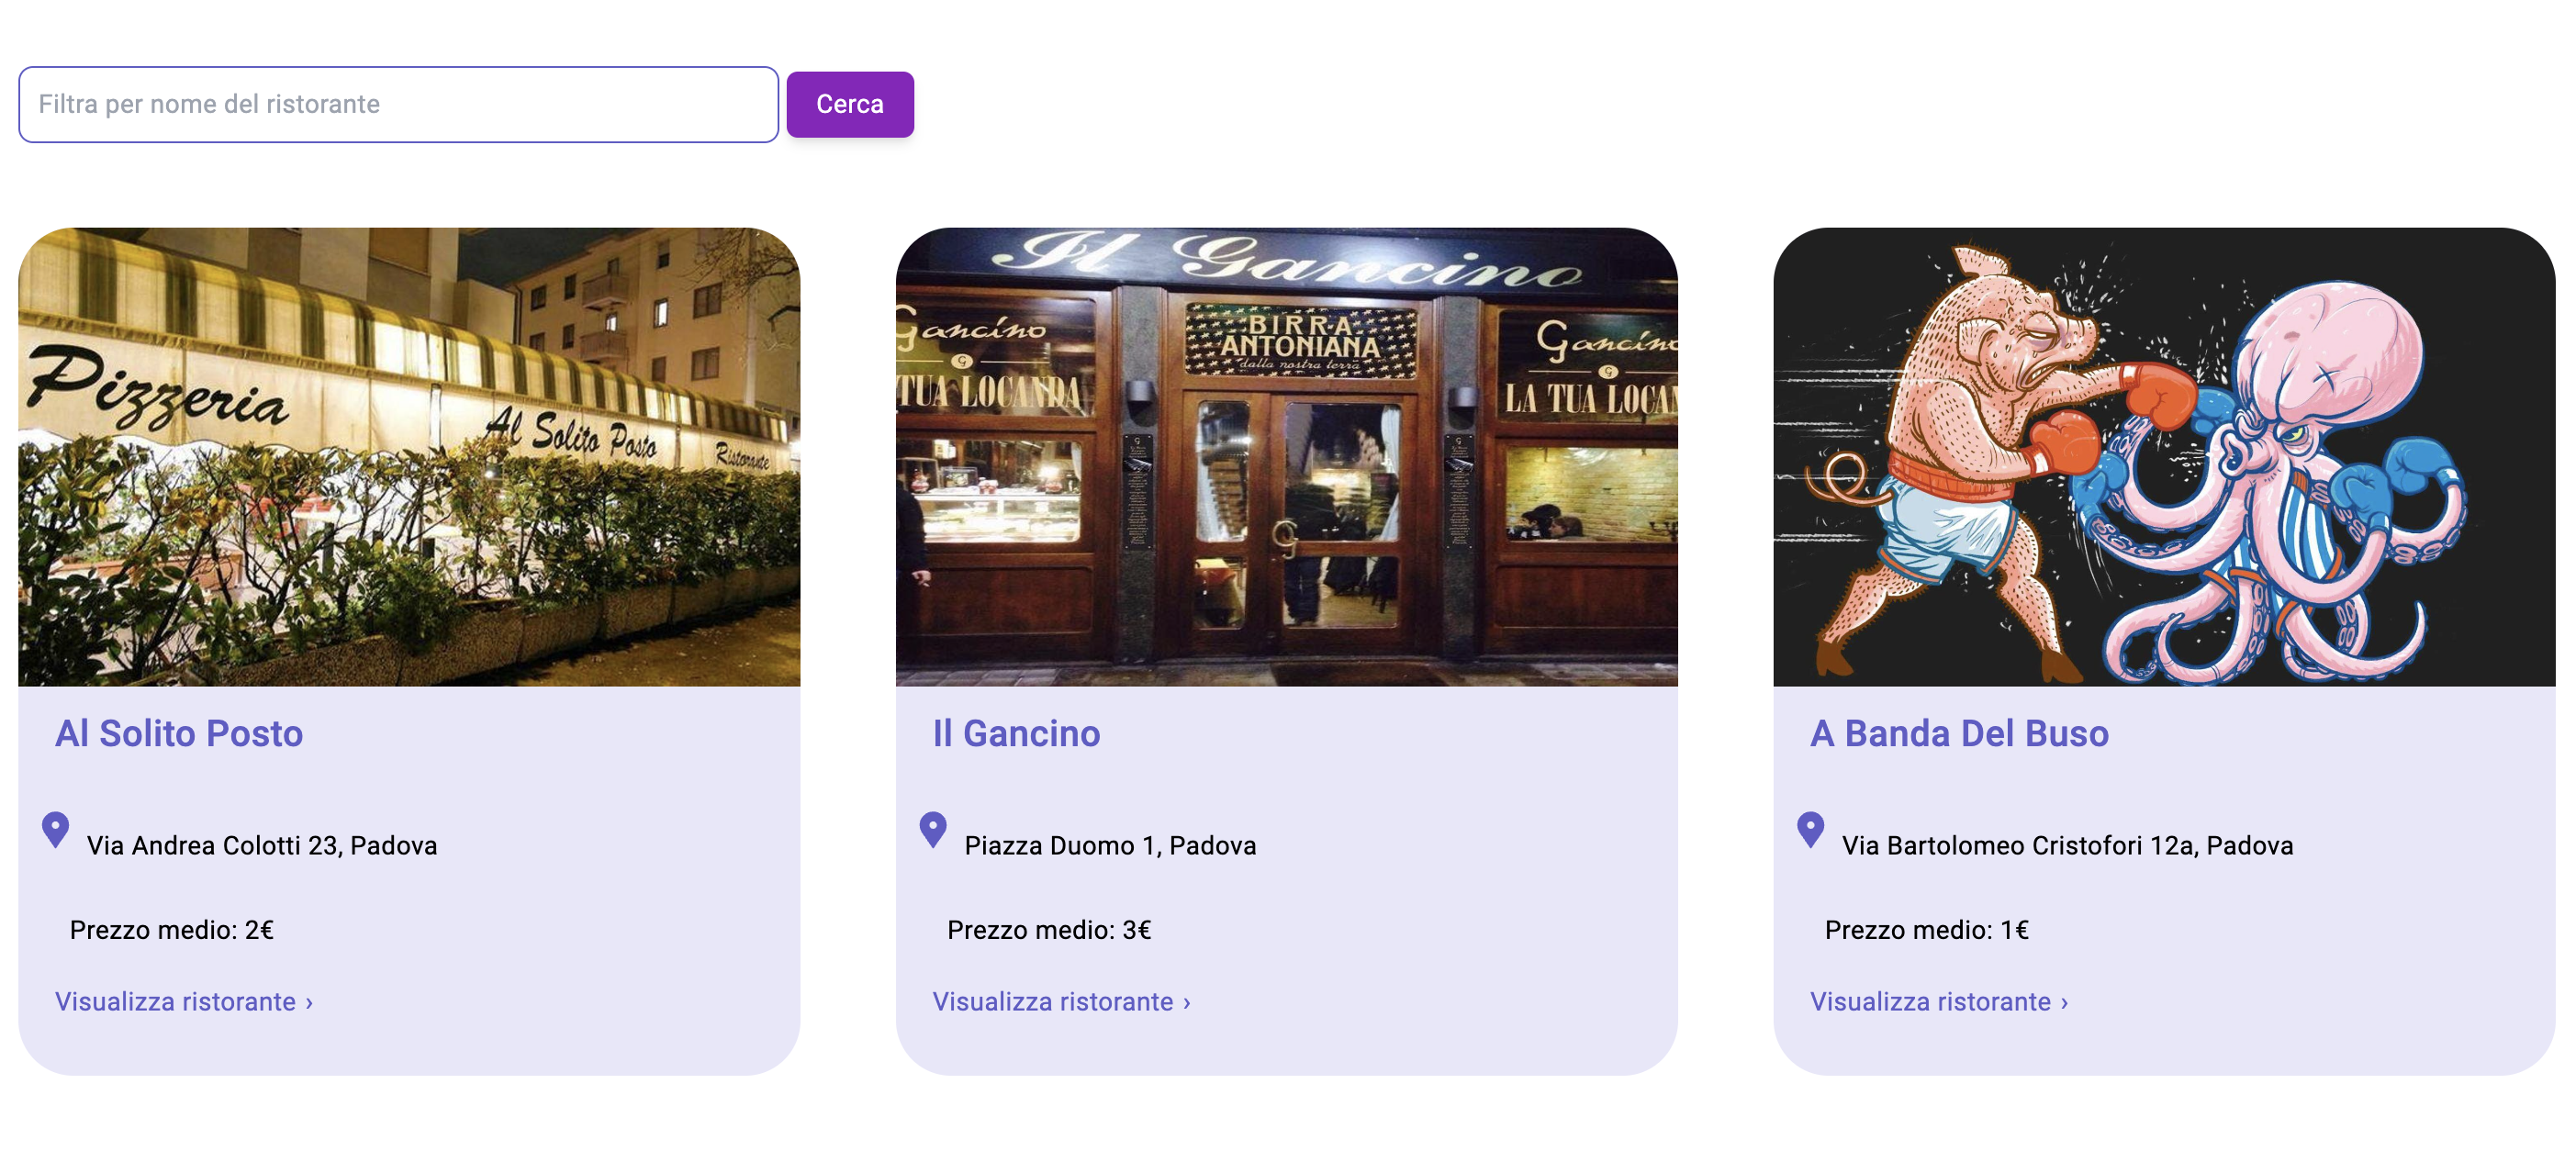
\includegraphics[width=0.8\textwidth]{PB/manuale-utente/home-non-autenticato.png}
    \caption{Home Page per l'utente non autenticato}
\end{figure}

La Home Page è il punto di ingresso principale per gli utenti non autenticati. 
Sono mostrati i ristorati presenti su EasyMeal e le loro informazioni
principali. In cima all'elenco è presente un campo di ricerca per trovare
rapidamente un ristorante conoscendone il nome. Infine, sotto a ciascun
ristorante è presente un riferimento cliccabile \texttt{Visualizza ristorante >}
che permette di visualizzare in dettaglio le informazioni del ristorante.

\subsection{Visualizza in dettaglio un ristorante}

\begin{figure}[htbp]
    \centering
	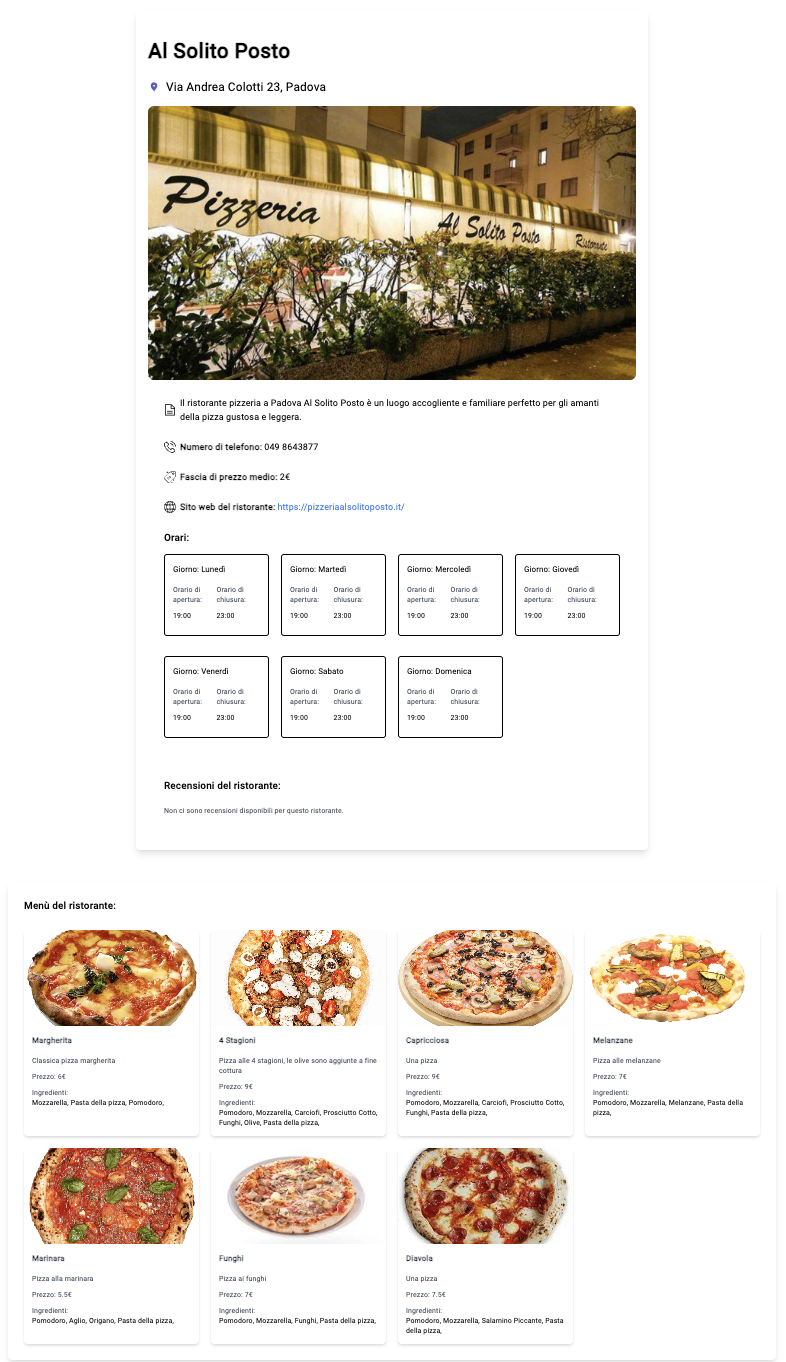
\includegraphics[width=0.6\textwidth]{PB/manuale-utente/dettagli-ristorante-non-autenticato.png}
    \caption{Pagina di visualizzazione in dettaglio di un ristorante per l'utente non autenticato}
\end{figure}
Nella seguente pagina sarà possibile visualizzare tutte le informazioni relative 
al ristorante ed il suo menù, con 
i relativi piatti e prezzi e inoltre è possibile visualizzare le recensioni del ristorante scritte dagli utenti.
Infine, copiando il \textit{link} del ristorante è possibile condividerlo con chiunque,
infatti questo \textit{link} è univoco per ogni ristorante e permette di accedere 
direttamente alla pagina di visualizzazione in dettaglio del ristorante.

\subsection{Login cliente}

\begin{figure}[htbp]
    \centering
	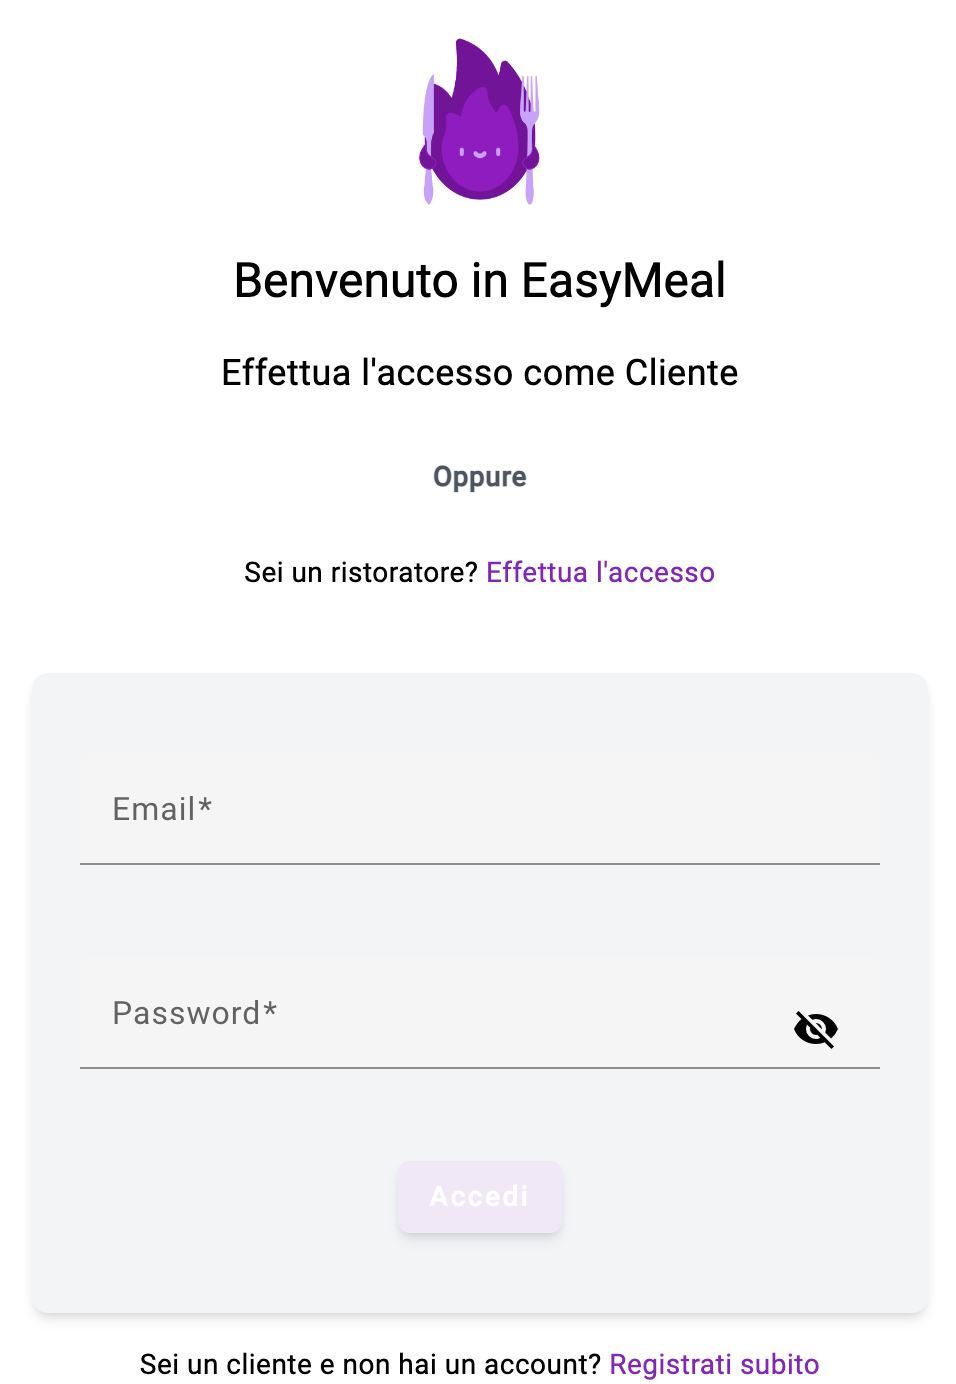
\includegraphics[width=0.3\textwidth]{PB/manuale-utente/login-cliente.png}
    \caption{Pagina di login lato utente cliente}
\end{figure}

In questa pagina è presente un \textit{form} di \textit{login} per permettere agli utenti di
accedere alle funzionalità di un cliente. In particolare, è necessario inserire
l'indirizzo \textit{email} e la \textit{password} corrispondente. Una volta inseriti i dati è
possible cliccare sul pulsante \texttt{Accedi} per procedere con 
l'autenticazione. Se l'autenticazione avviene con successo, verrà mostrata una
notifica in basso a destra indicante "Utente autenticato". Se ci sono errori
durante l'autenticazione verrà mostrato un messaggio di errore appropriato.\\
In cima al \textit{form}, è presente un \textit{link} cliccabile "Sei un ristoratore?
\texttt{Effettua l'accesso}" che permette di accedere alla pagina di \textit{login} per
i ristoratori. In fondo al \textit{form}, è presente un link cliccabile "Sei un cliente e 
non hai un account? \texttt{Registrati}" che permette di accedere alla pagina di 
registrazione per gli utenti clienti.

\subsection{Login ristoratore}

La pagina di \textit{login} del ristoratore è analoga a quella del cliente. In
particolare è possibile accedere alla pagina di \textit{login} per i ristoratori 
cliccando sul link "Sei un ristoratore? \texttt{Effettua l'accesso}" presente 
nella pagina di \textit{login} per i clienti, oppure cliccando sul \textit{link} 
"Login ristoratori" presente nel \textit{footer} di ogni pagina.

\subsection{Registrazione cliente}

\begin{figure}[htbp]
    \centering
	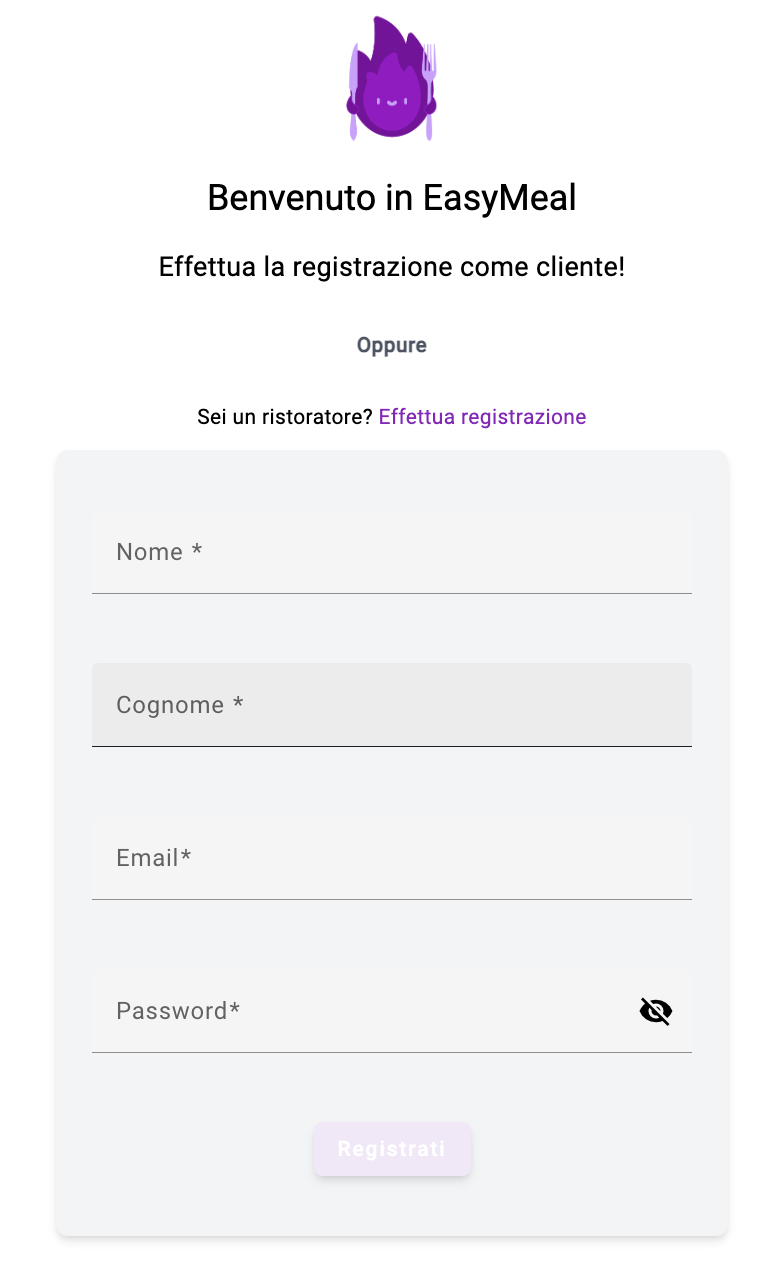
\includegraphics[width=0.3\textwidth]{PB/manuale-utente/registrazione-cliente.png}
    \caption{Pagina di registrazione lato utente cliente}
\end{figure}

Per registrarti come nuovo cliente, compila il \textit{form} di registrazione con le
seguenti infomazioni:

\begin{itemize}
	\item Nome e cognome;
	\item Indirizzo \textit{email};
	\item \textit{Password};
\end{itemize}

Una volta completata la compilazione del \textit{form} e inviata la richiesta di registrazione, riceverai 
una notifica in basso a destra indicante 
``Utente creato con successo'' se la registrazione è avvenuta con successo.
Altrimenti, è visualizzato un messaggio di errore se ci sono problemi durante il
processo di registrazione.\\
In cima al form di registrazione, è presente un \textit{link} "Sei un ristoratore?
\texttt{Effettua la registrazione}" che permette di accedere alla pagina di
registrazione per i ristoratori.

\newpage
\subsection{Registrazione ristoratore}

\begin{figure}[htbp]
    \centering
	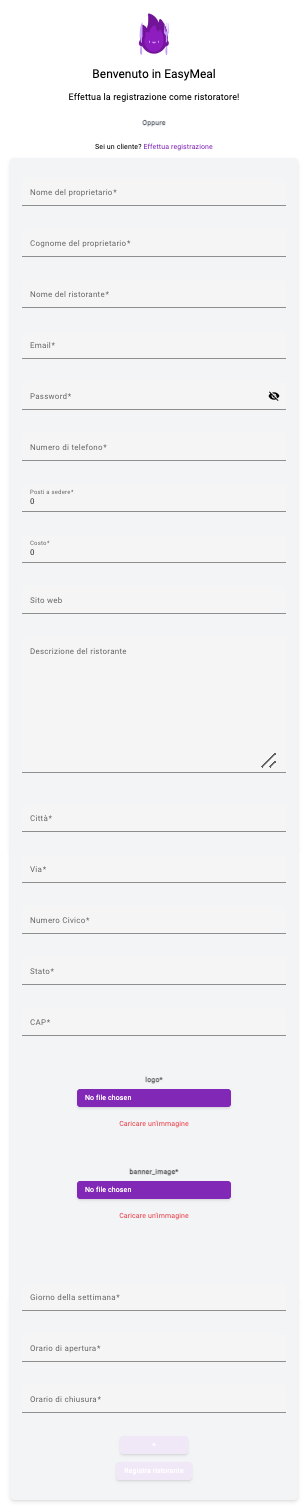
\includegraphics[width=0.3\textwidth]{PB/manuale-utente/registrazione-ristoratore.png}
    \caption{Pagina di registrazione lato utente cliente}
\end{figure}

Per registrarti come nuovo ristoratore, compila il \textit{form} di registrazione con le
seguenti informazioni:
\begin{itemize}
	\item Nome e cognome del proprietario;
	\item Nome del ristorante;
	\item Indirizzo \textit{email};
	\item \textit{Password};
	\item Numero di telefono;
	\item Posti a sedere;
	\item Costo (da 0 a 3, dove 0 è il minimo e 3 il massimo);
	\item Indirizzo del sito \textit{web} del ristorante (opzionale);
	\item Descrizione del ristorante (opzionale);
	\item Città;
	\item Via;
	\item Numero civico;
	\item Stato;
	\item CAP;
	\item Il logo del ristorante;
	\item Il banner del ristorante;
	\item Orari di apertura e chiusura per ciascun giorno della settimana.
\end{itemize}

Una volta completata la compilazione del \textit{form} e inviata la richiesta di registrazione, riceverai 
una notifica in basso a destra che indica il successo o il fallimento
dell'operazione.

In particolare, dopo aver compilato il \textit{form} di inserimento di un giorno con
relativo orario di apertura e chiusura, è possibile cliccare sul pulsante
\texttt{+} per aggiungere un altro giorno. Una volta aggiunto un orario, è
possibile rimuoverlo cliccando sul pulsante \texttt{X} a destra del suddetto
orario.\\
In cima al \textit{form} di registrazione, è presente un \textit{link} "Sei un cliente? \texttt{Effettua la registrazione}"


\subsection{Cliente} % --------------------- SECTION DEL CLIENTE ---------------------%

 
\subsubsection{Home Page}
Una volta effettuato l'accesso come cliente, verrai reindirizzato alla tua Home Page personale.
Questa Home Page è praticamente identica a quella degli utenti non autenticati, ma con modifiche 
relative alla barra di navigazione in alto. 


\subsection{Barra di navigazione}
La barra di navigazione in alto ti permette di accedere alle sezioni di esplorazione dei ristoranti, 
visualizzare e gestire le proprie prenotazioni, controllare e leggere le notifiche ricevute ed effettuare il ``logout''.

\subsubsection{Esplora}
La sezione ``Esplora'' ti permette di cercare, filtrare e visualizzare tutti i ristoranti registrati su EasyMeal, 
e andare in dettaglio per visualizzare tutte le informazioni relative ad un ristorante. Esattamente come un utente non autenticato.

Una volta entrati nel dettaglio di un ristorante, c'è un'aggiunta speciale: il bottone ``Prenota'' che ti permette di prenotare un tavolo di un ristorante, 
se c'è ancora disponibilità di posti a sedere.

\begin{figure}[htbp]
	\centering
	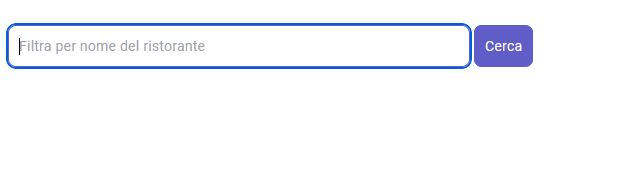
\includegraphics[width=0.5625\textwidth]{./img/Dettaglio.jpg}
	\caption{Bottone di prenotazione di un tavolo di un ristorante}
	% \label{fig:esempio8}
\end{figure}

\subsubsection{Prenotazione di un tavolo}
Una volta cliccato sul tasto prenotazione di un tavolo comparirà un form per inviare la richiesta di prenotazione che sarà accettata o rifiutata dal ristoratore.
Sarà richiesto di inserire il giorno desiderato e un orario compreso tra l'orario di apertura e chiusura del ristorante di quel relativo giorno, inoltre il numero 
di persone che saranno presenti al tavolo.

\begin{figure}[htbp]
	\centering
	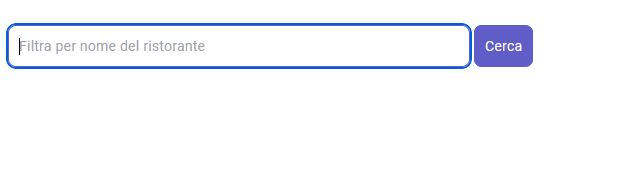
\includegraphics[width=0.5625\textwidth]{./img/Dettaglio.jpg}
	\caption{Form di richiesta di prenotazione di un tavolo di un ristorante}
   %  \label{fig:esempio9}
\end{figure}

\subsubsection{Gestione prenotazioni}
Tornando alla barra di navigazione, cliccando su ``Prenotazioni'' si accede alla pagina di gestione delle prenotazioni.
In cui si ha un elenco di tutte le prenotazioni effettuate, con la possibilità di visualizzare in dettaglio una prenotazione, semplicemente cliccando su di essa.
In questa lista si possono visualizzare le prenotazioni in attesa di conferma, quelle confermate e quelle rifiutate, quindi si possono visualizzare il nome della 
prenotazione, l'orario in cui è stata effettuata, lo stato della prenotazione e il ristorante a cui si riferisce, e lo stato della prenotazione.

\begin{figure}[htbp]
	\centering
	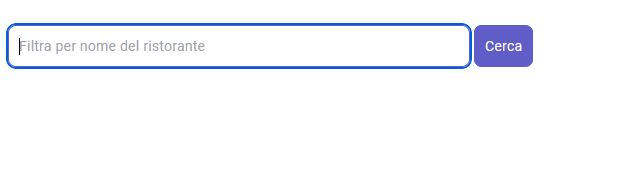
\includegraphics[width=0.5625\textwidth]{./img/Dettaglio.jpg}
	\caption{Visualizzazione delle prenotazioni effettuate}
	% \label{fig:esempio10}
\end{figure}

\subsubsection{Eliminazione prenotazione}
Nel caso in cui si è stati aggiunti ad un prenotazione e non si vuole partecipare o la si vuole cancellare bisognerà semplicemente cliccare sul pulsante ``X'' 
che compare a destra di ciascuna prenotazione nella lista.

\begin{figure}[htbp]
	\centering
	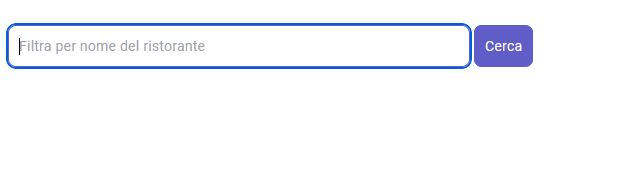
\includegraphics[width=0.5625\textwidth]{./img/Dettaglio.jpg}
	\caption{Pulsante di eliminazione di una prenotazione}
	% \label{fig:esempio11}
\end{figure}

\subsubsection{Accettazione prenotazione}
Nel caso contrario, ovvero nel caso in cui si è stati aggiunti ad una prenotazione e si desidera confermare la presenza bisognerà semplicemente cliccare sul pulsante ``V'', 
che compare a destra di ciascuna prenotazione nella lista.

\begin{figure}[htbp]
	\centering
	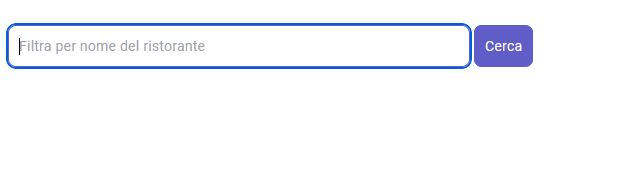
\includegraphics[width=0.5625\textwidth]{./img/Dettaglio.jpg}
	\caption{Pulsante di accettazione di una prenotazione}
	% \label{fig:esempio12}
\end{figure}

\subsubsection{Notifiche}
Tornando alla barra di navigazione, cliccando su ``Notifiche'' si accede alla pagina di visualizzazione delle notifiche.
In cui si ha la possibilità di filtrare le notifiche in base a Nuove o Lette, semplicemente cliccando sopra nuove o lette. Per default 
saranno visualizzate quelle nuove in base all'ordine di ricezione. 
Per eliminare la spunta di novità su una notifica basterà cliccare su di essa.

\begin{figure}[htbp]
	\centering
	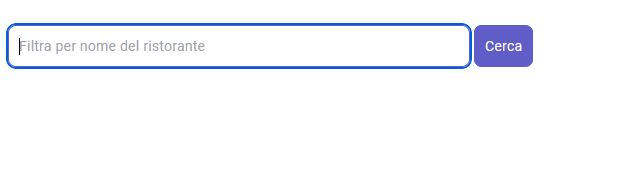
\includegraphics[width=0.5625\textwidth]{./img/Dettaglio.jpg}
	\caption{Visualizzazione delle notifiche ricevute}
	% \label{fig:esempio13}
\end{figure}

\subsubsection{Logout}
L'ultima funzionalità presente nella barra di navigazione di un cliente è la possibilità di effettuare il ``logout'' cliccando sul pulsante ``Logout''.
Una volta effettuato con successo si sarà reindirizzati nella Home Page di un classico utente non autenticato con le relative funzionalità.

\section{Ristoratore}

\subsection{Header}

\begin{figure}[htbp]
    \centering
	
\includegraphics[width=1\textwidth]{PB/manuale-utente/header-ristoratore.png}
    \caption{Barra di Navigazione per il ristoratore}
\end{figure}

La barra di navigazione in alto ti permette di accedere facilmente alle varie 
sezioni della piattaforma:
\begin{itemize}
	\item \texttt{Logo e "Easy Meal"}: cliccando sul logo o sul nome "Easy Meal"
		sei reindirizzato alla Home Page della piattaforma;

	\item \texttt{Esplora}: cliccando su questo riferimento sei reindirizzato
		alla Home Page della piattaforma;

	\item \texttt{Ingredienti}: cliccando su questa voce sei reindirizzato alla
		pagina di gestione degli ingredienti del tuo ristorante;

	\item \texttt{Piatti}: cliccando su questo riferimento sei reindirizzato
		alla pagina di visualizzazione dei piatti del tuo ristorante;

	\item \texttt{Prenotazioni}: cliccando su questo riferimento sei 
		reindirizzato alla pagina di visualizzazione della lista di
		prenotazioni;

	\item \texttt{Notifiche}: cliccando su questo riferimento sei reindirizzato
		alla pagina di visualizzazione della lista di notifiche. Nota che se ci
		sono notifiche non lette, il riferimento sarà seguito da un \textit{badge} che
		indica il numero di notifiche non lette;

	\item \texttt{Logout}: cliccando su questo riferimento effettuerai il \textit{logout}
		dalla piattaforma e sarai reindirizzato alla Home Page della 
		piattaforma.
\end{itemize}

\subsection{Esplora (Home Page)}

Questa pagina è analoga alla Home Page della piattaforma per l'utente generico.

\subsection{Ingredienti}

\begin{figure}[htbp]
    \centering
	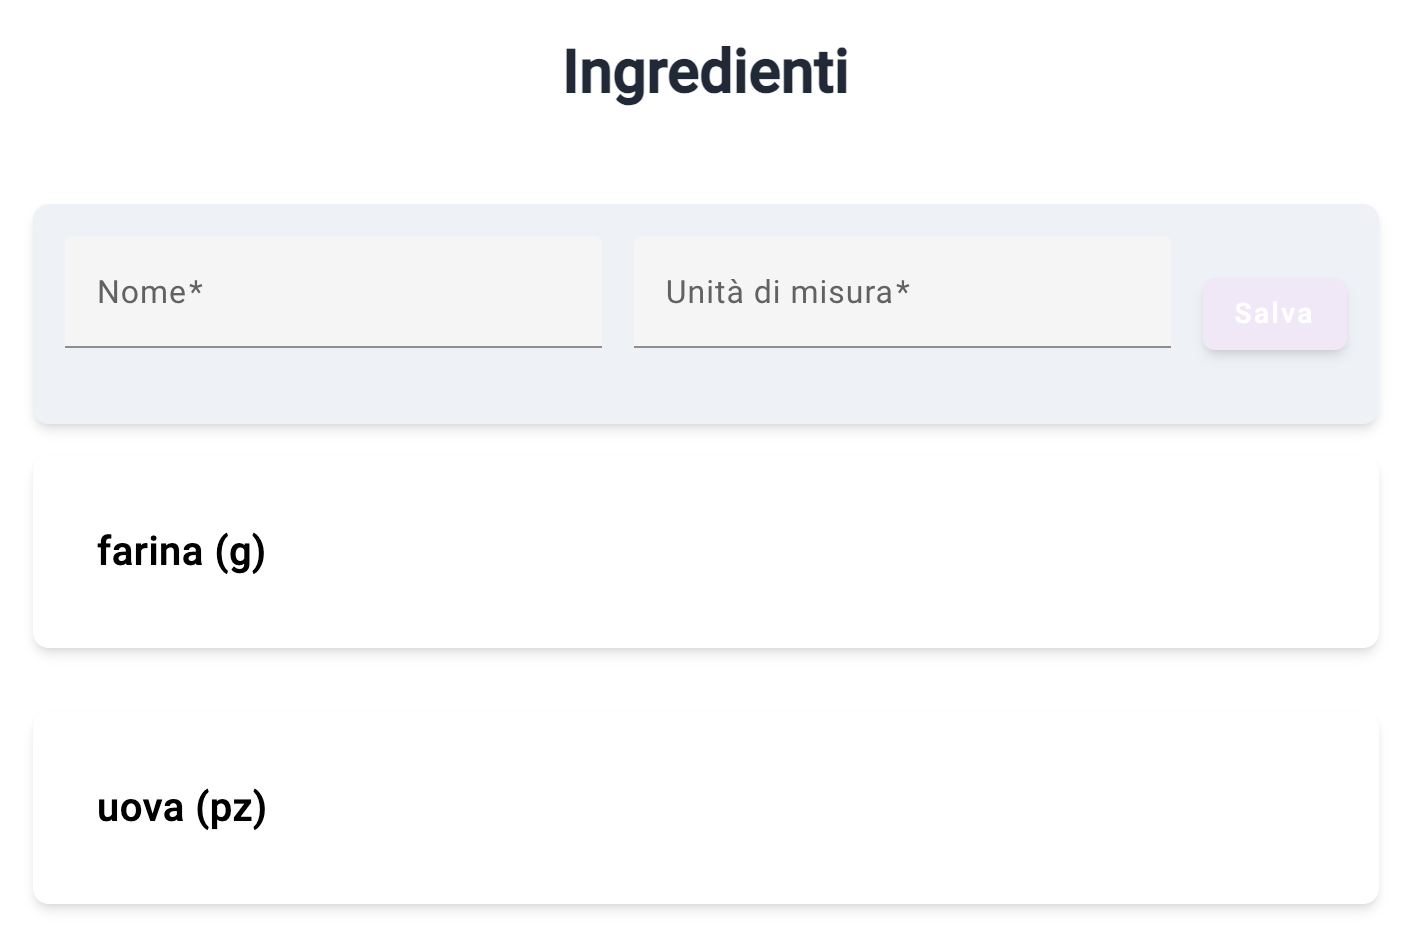
\includegraphics[width=0.8\textwidth]{PB/manuale-utente/ingredienti-ristoratore.png}
    \caption{Pagina di visualizzazione delle prenotazioni per il ristoratore}
\end{figure}

Si accede a questa pagina cliccando su \texttt{Ingredienti} nella barra di
navigazione. Qui puoi visualizzare tutti gli ingredienti presenti nel menu del
tuo ristorante. In cima alla lista degli ingredienti è presente un modulo che
richiede:
\begin{itemize}
	\item Nome: il nome dell'ingrediente;
	\item Unità di misura: l'unità di misura dell'ingrediente. Le opzioni
		disponibili sono: g, ml, p, q.b.
\end{itemize}

Avendo compilato i campi, puoi salvare l'ingrediente cliccando sul pulsante
\texttt{Salva}. Viene visualizzato un messaggio di conferma o di errore
dell'operazione. Sotto il modulo di inserimento sono elencati tutti gli
ingredienti presenti nel menu del ristorante. Puoi modificarli cliccando su di
un ingrediente. Dopo aver cliccato su un ingrediente, esso si trasforma in un
\textit{form} che ti permette di modificare i campi dell'ingrediente. Puoi eliminare
l'ingrediente cliccando sul pulsante \texttt{Elimina} a destra, oppure lo puoi
salvare cliccando sul pulsante \texttt{Salva}.

\subsection{Piatti}

\begin{figure}[htbp]
    \centering
	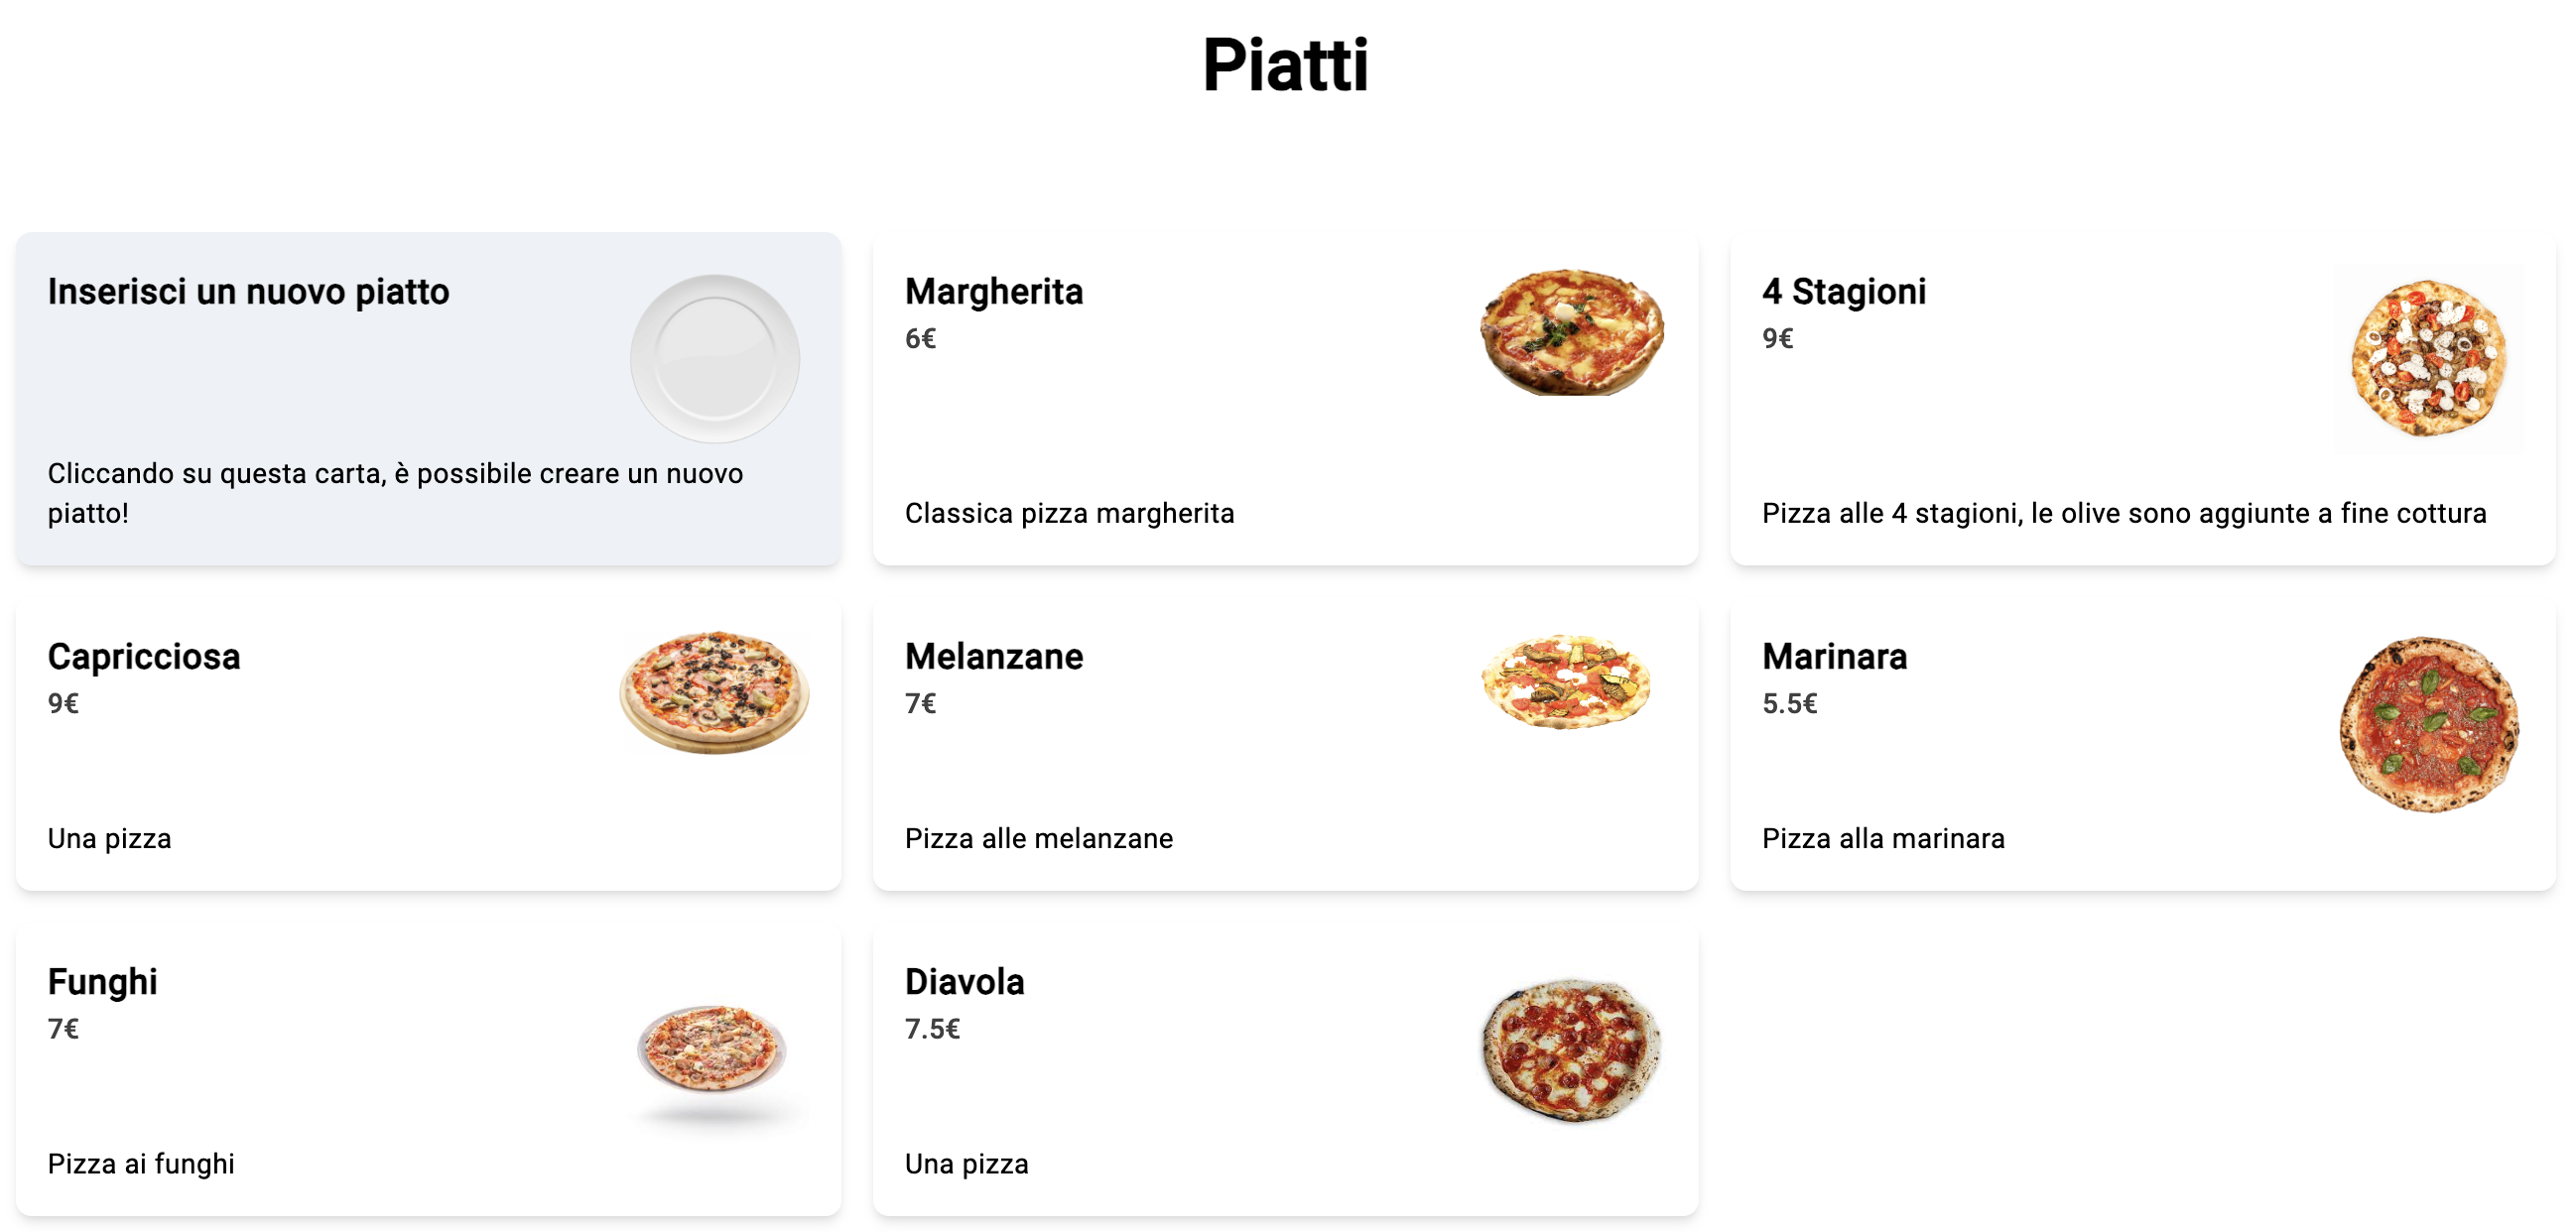
\includegraphics[width=1\textwidth]{PB/manuale-utente/piatti-ristoratore.png}
    \caption{Pagina di visualizzazione dei piatti per il ristoratore}
\end{figure}

Si accede a questa pagina cliccando su \texttt{Piatti} nella barra di
navigazione. Qui puoi visualizzare tutti i piatti presenti nel menu del tuo
ristorante. Cliccando su di un piatto si accede alla pagina di dettaglio del
piatto. Cliccando sul primo piatto della lista si accede alla pagina di
inserimento di un nuovo piatto.

\newpage
\subsection{Nuovo piatto}

\begin{figure}[htbp]
    \centering
	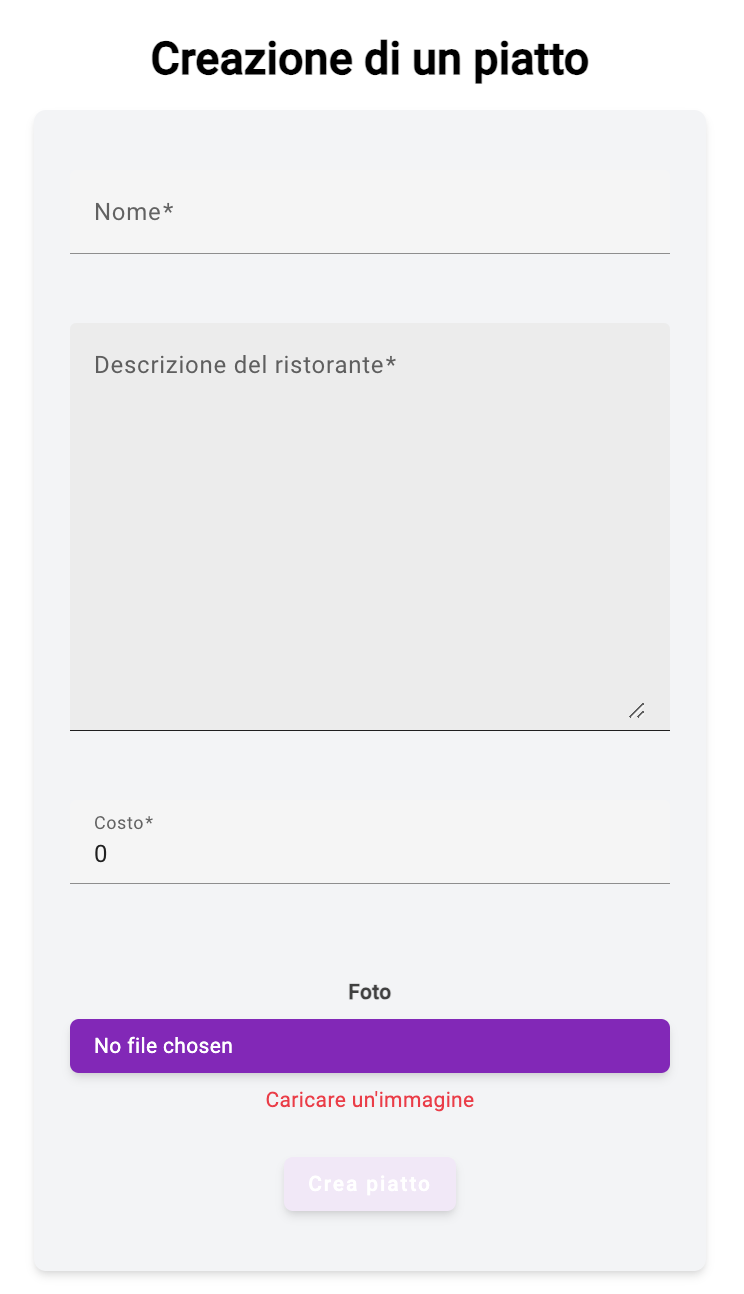
\includegraphics[width=0.6\textwidth]{PB/manuale-utente/nuovo-piatto-ristoratore.png}
    \caption{Pagina di inserimento di un nuovo piatto per il ristoratore}
\end{figure}

Si accede a questa pagina cliccando sul primo piatto della lista dei piatti.
Questa pagina è composta da un \textit{form} che richiede:
\begin{itemize}
	\item Nome;
	\item Descrizione del piatto;
	\item Costo;
	\item Foto.
\end{itemize}

Dopo aver compilato il \textit{form}, puoi salvare il piatto cliccando sul pulsante
\texttt{Crea piatto}. Se l'operazione va a buon fine, vieni reindirizzato alla
pagina di dettaglio del piatto e viene visualizzato un messaggio di conferma di
avvenuta creazione del piatto, altrimenti viene visualizzato un messaggio di
errore.

\subsection{Dettaglio piatto}

\begin{figure}[htbp]
    \centering
	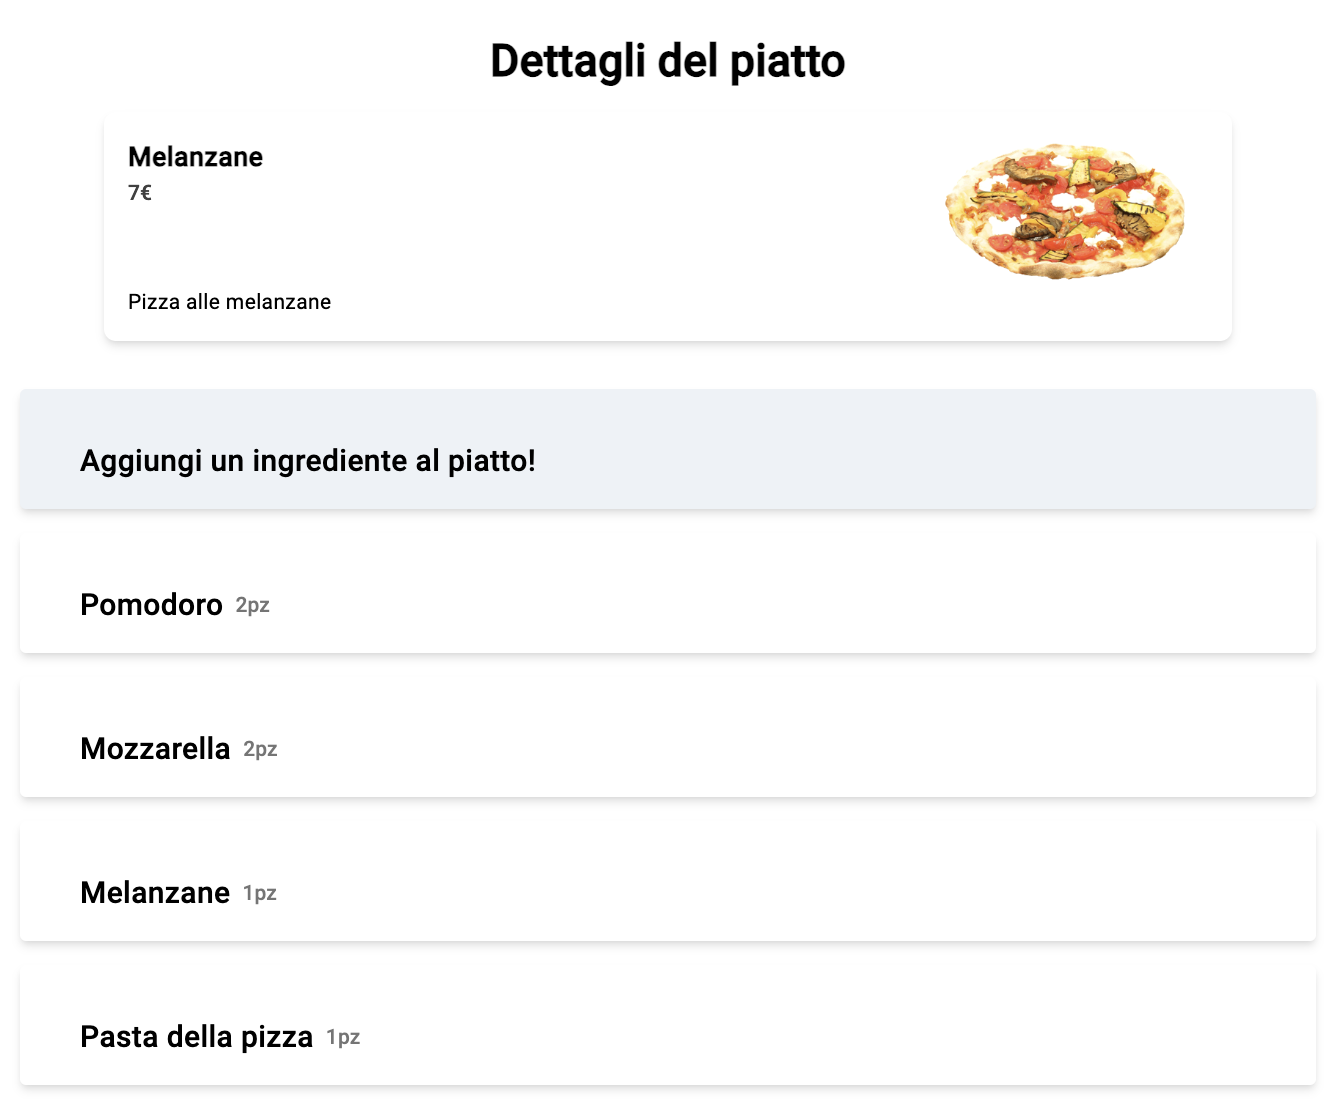
\includegraphics[width=0.8\textwidth]{PB/manuale-utente/dettaglio-piatto-ristoratore.png}
    \caption{Pagina di dettaglio di un piatto per il ristoratore}
\end{figure}

Si accede a questa pagina cliccando su un piatto nella lista dei piatti. Qui
puoi visualizzare i dettagli del piatto e i suoi ingredienti. In questa pagina
sono disponibili le seguenti funzionalità:
\begin{itemize}
	\item \textbf{Modifica piatto}: cliccando sul piatto, esso si trasforma
		nel \textit{form} di creazione con i campi già compilati. Puoi modificare i
		campi e salvare le modifiche cliccando sul pulsante \texttt{Modifica
		piatto}. Se l'operazione va a buon fine, vieni reindirizzato alla
		pagina di visualizzazione dei piatti e viene visualizzato un messaggio
		di conferma di avvenuta modifica del piatto, altrimenti viene
		visualizzato un messaggio di errore;

	\item \textbf{Elimina piatto}: cliccando sul piatto, esso si trasforma nel
		\textit{form} di creazione con i campi già compilati. In fondo al \textit{form} è presente
		un bottone \texttt{Elimina piatto}. Cliccando su questo bottone, il
		piatto viene eliminato. Viene visualizzato un messaggio di conferma e
		vieni reindirizzato alla pagina di visualizzazione dei piatti; altrimenti 
		viene visualizzato un messaggio di errore dell'operazione;

	\item \textbf{Aggiungi ingrediente}: sotto ad ogni piatto è presente un
		pulsante \texttt{Aggiungi un ingrediente al piatto}. Cliccando su
		questo pulsante si apre un \textit{form} che ti permette di aggiungere un
		ingrediente al piatto. Il \textit{form} richiede:
		\begin{itemize}
			\item Ingrediente: un ingrediente presente negli ingredienti del tuo
				ristorante. Cliccando su questo campo si apre un menu a
				tendina con tutti gli ingredienti presenti nel tuo ristorante;

			\item Quantità: la quantità dell'ingrediente da aggiungere al piatto.
		\end{itemize}
		Dopo aver compilato il \textit{form}, puoi salvare l'ingrediente cliccando sul
		pulsante \texttt{Aggiungi ingrediente}. Se l'operazione va a buon fine,
		viene visualizzato un messaggio di conferma di avvenuta aggiunta
		dell'ingrediente al piatto, altrimenti viene visualizzato un messaggio
		di errore;

	\item \textbf{Modifica di un ingregrediente del piatto}: sotto al pulsante
		di aggiunta di un ingrediente è presente un elenco degli ingredienti
		del piatto. Cliccando su un ingrediente si apre un \textit{form} che ti permette
		di modificare la quantità dell'ingrediente dal piatto. Dopo aver 
		modificato la quantità
		dell'ingrediente, puoi salvare le modifiche cliccando sul pulsante
		\texttt{Modifica ingrediente}. Se l'operazione va a buon fine, viene visualizzato un
		messaggio di conferma di avvenuta modifica dell'ingrediente, altrimenti
		viene visualizzato un messaggio di errore;

	\item \textbf{Elimina ingrediente}: sotto al pulsante di aggiunta di un
		ingrediente è presente un elenco degli ingredienti del piatto. Cliccando
		su un ingrediente si apre un \textit{form} che ti permette di modificare la
		quantità dell'ingrediente dal piatto. In fondo al \textit{form} è presente un
		bottone \texttt{Elimina ingrediente}. Cliccando su questo bottone,
		l'ingrediente viene eliminato dal piatto. Viene visualizzato un messaggio
		di conferma e viene visualizzato un messaggio di conferma di avvenuta
		eliminazione dell'ingrediente dal piatto, altrimenti viene visualizzato
		un messaggio di errore dell'operazione.
\end{itemize}

\subsection{Prenotazioni}

\begin{figure}[htbp]
    \centering
	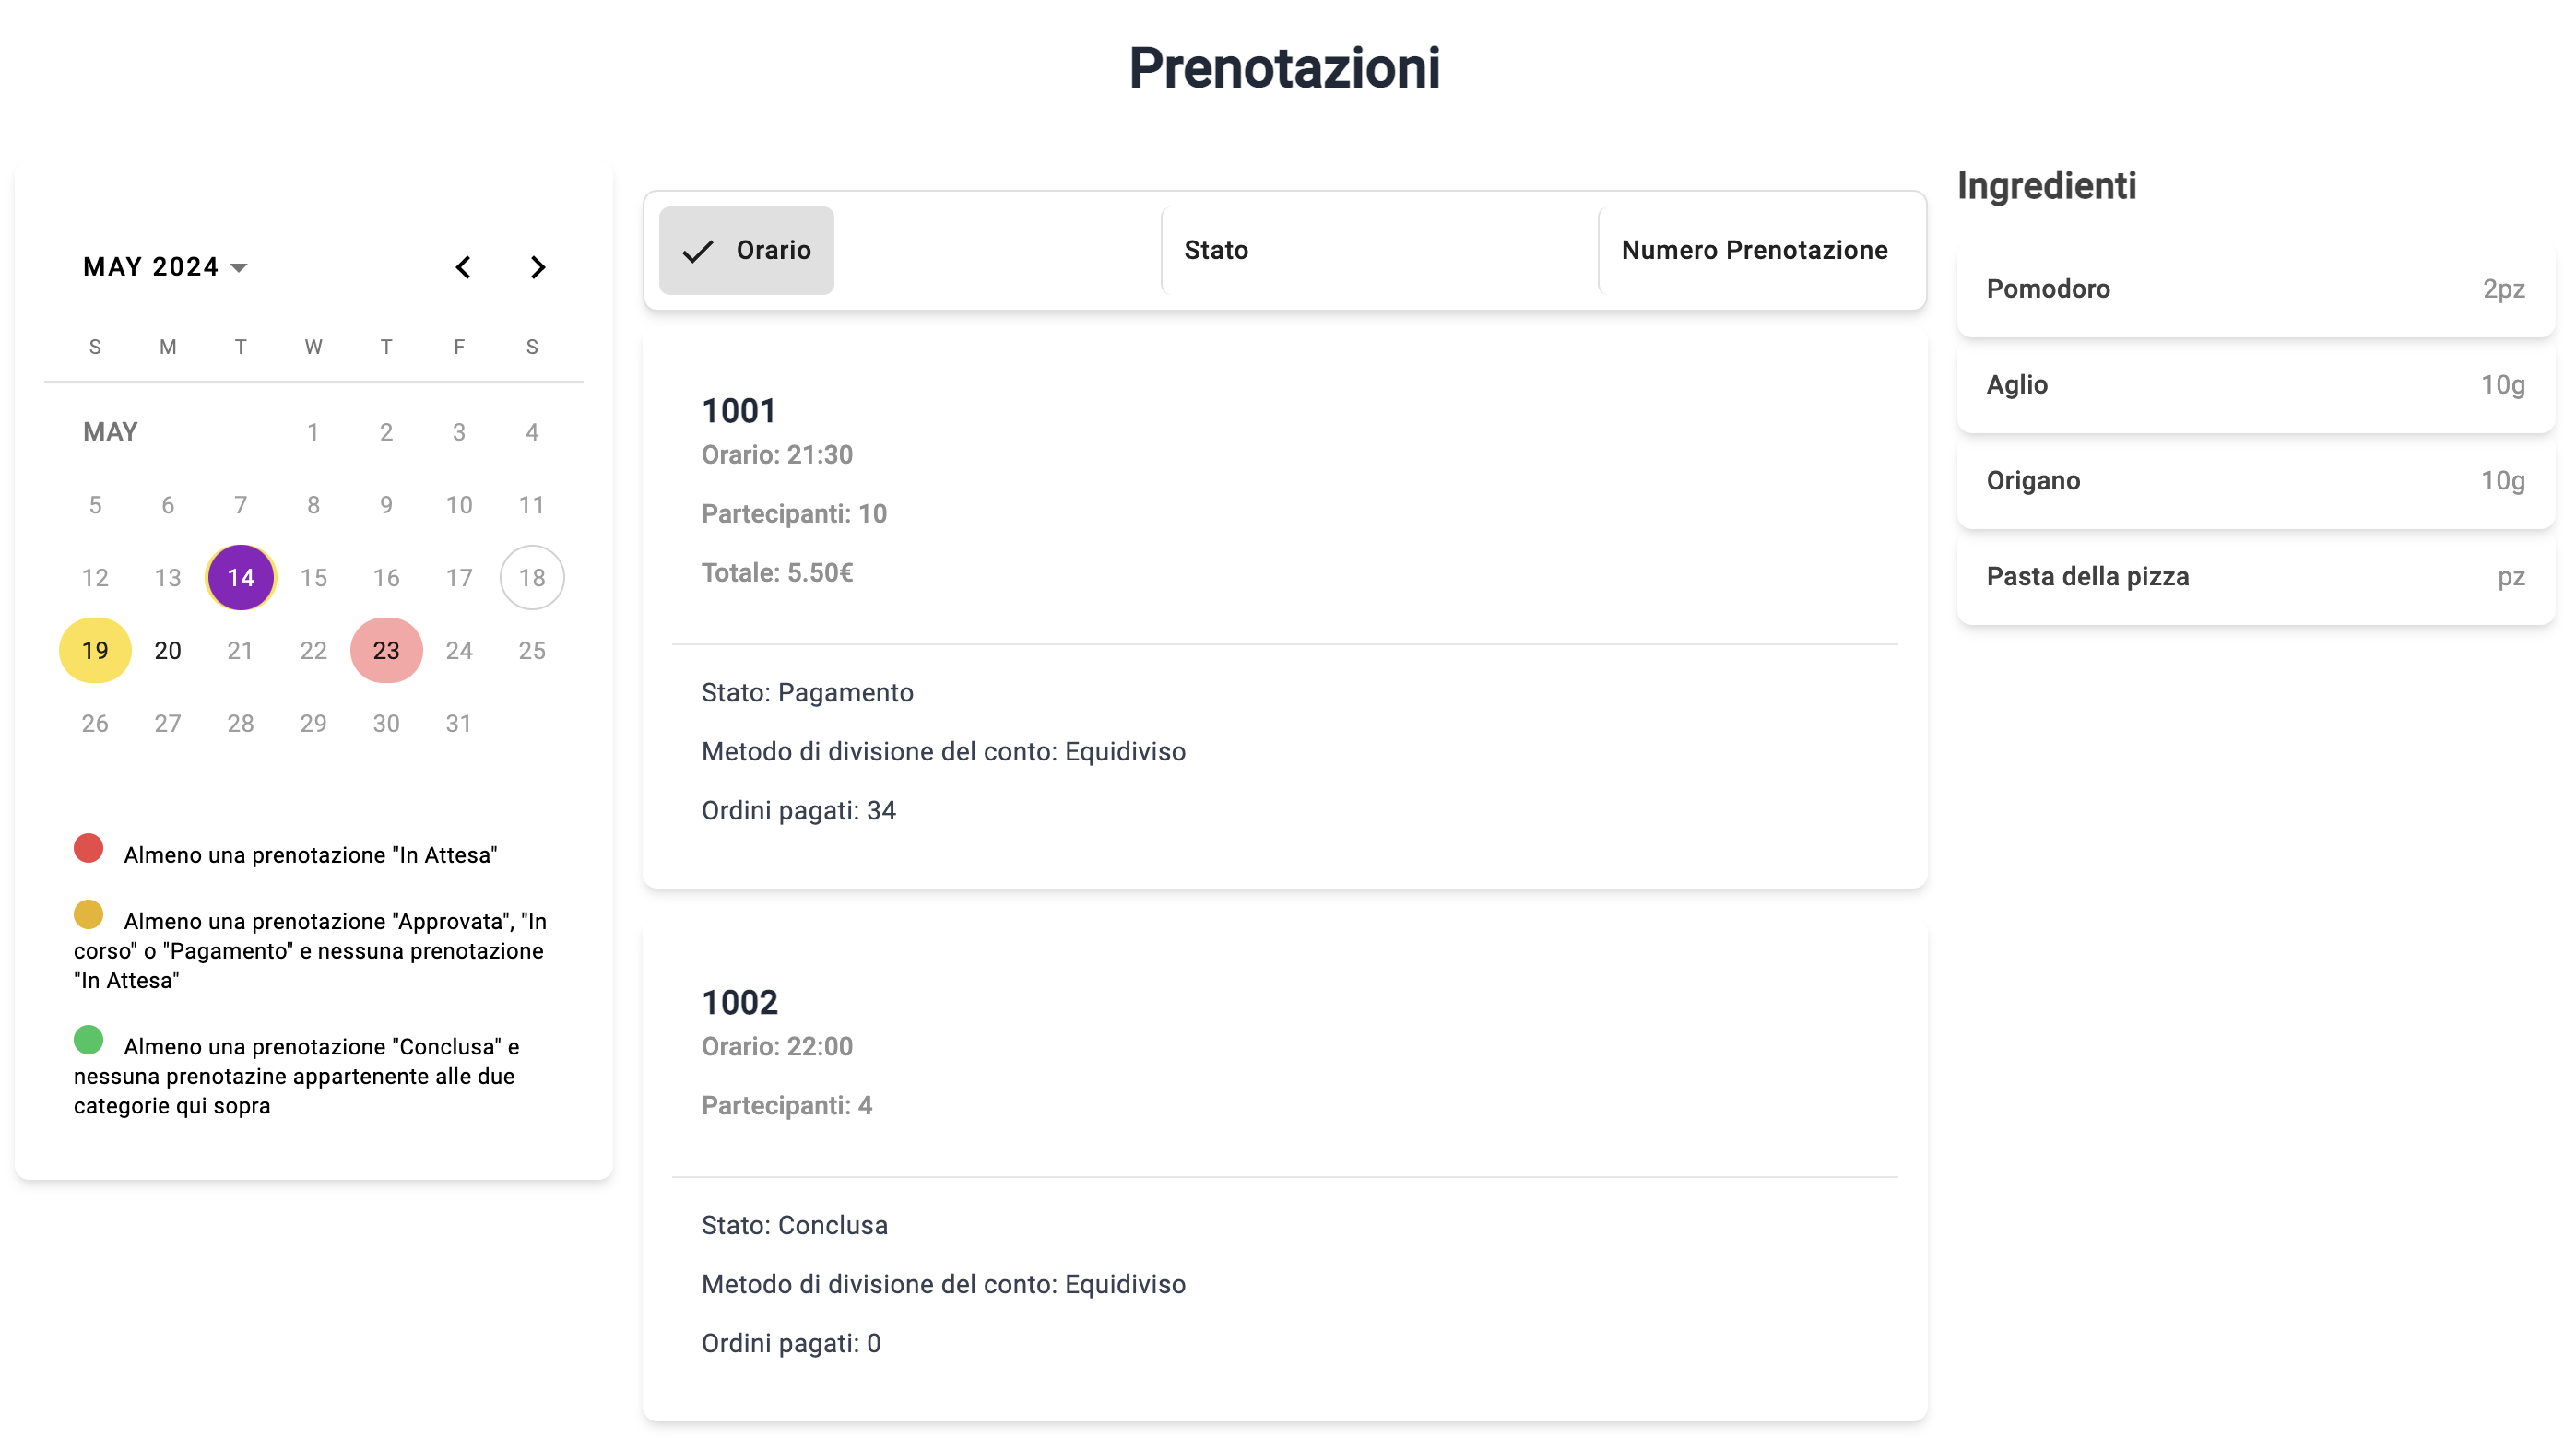
\includegraphics[width=1\textwidth]{PB/manuale-utente/prenotazioni-ristoratore.png}
	\caption{Pagina di visualizzazione delle prenotazioni per il ristoratore}
\end{figure}

Si accede a questa pagina cliccando su \texttt{Prenotazioni} nella barra di
navigazione. La pagina delle prenotazioni è divisa in tre sezioni:
\begin{itemize}
	\item \textbf{Calendario}: questa sezione occupa la parte sinistra della pagina. Qui è possibile selezionare un giorno e visualizzare i colori dei giorni e la loro cliccabilità. I giorni colorati in rosso indicano che c'è almeno una prenotazione nello stato "In attesa", il che significa che devi ancora confermare la disponibilità. I giorni colorati in giallo indicano che non ci sono prenotazioni "In attesa", ma almeno una è nello stato "Approvata", "In corso" o "Pagamento". I giorni colorati in verde indicano che non ci sono prenotazioni nelle categorie precedenti, ma almeno una è nello stato "Conclusa". I giorni cliccabili, ma non colorati, hanno solo prenotazioni nello stato "Rifiutata" o "Annullata". Selezionando un giorno del calendario, si aggiorna la lista delle prenotazioni in base al giorno scelto;
	\item \textbf{Lista delle prenotazioni}: 
	questa è la sezione centrale della pagina. Qui sono elencate tutte le prenotazioni relative al giorno selezionato nel calendario. Cliccando su una prenotazione, verrai reindirizzato alla pagina di dettaglio della prenotazione. In cima alla lista delle prenotazioni ci sono tre pulsanti per riordinare le prenotazioni in base a: \texttt{Orario}, \texttt{Stato} e \texttt{Numero prenotazione}. Cliccando su uno di questi pulsanti, le prenotazioni verranno riordinate in base al campo selezionato;
	\item \textbf{Lista degli ingredienti}: 
	questa sezione occupa la parte destra della pagina. Qui sono elencati tutti gli ingredienti necessari per soddisfare le prenotazioni del giorno selezionato. Si noti che le prenotazioni "Annullata" e "Rifiutata" non sono considerate, mentre le prenotazioni "In attesa" sono incluse.
\end{itemize}

\subsection{Dettaglio prenotazione}

\begin{figure}[htbp]
    \centering
	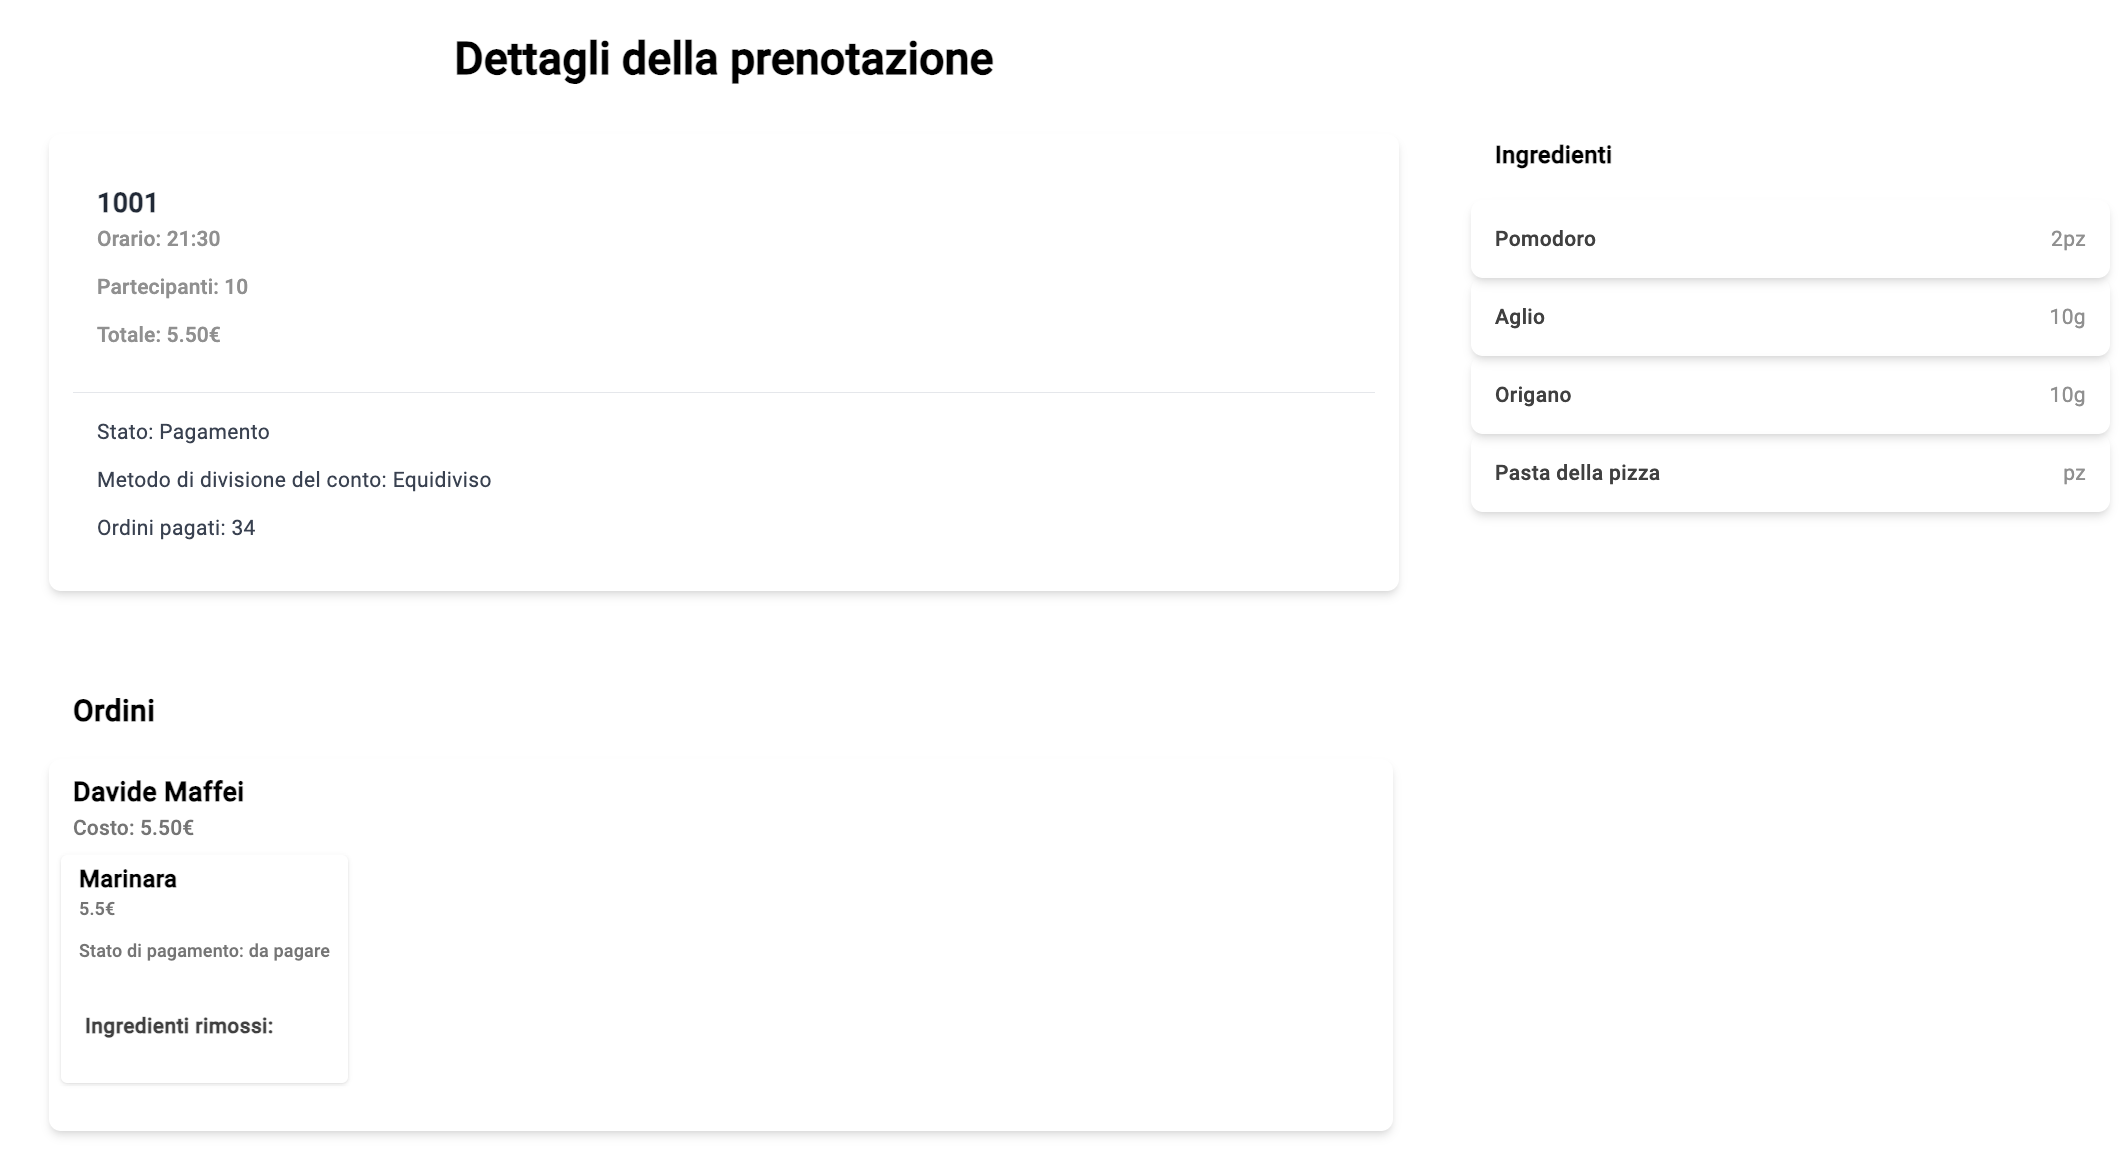
\includegraphics[width=1\textwidth]{PB/manuale-utente/dettaglio-prenotazione-ristoratore.png}
    \caption{Pagina di dettaglio di un'ordinazione per il ristoratore}
\end{figure}

Si accede a questa pagina cliccando su una prenotazione nella lista delle prenotazioni. Qui puoi visualizzare i dettagli della prenotazione e i piatti ordinati. Cliccando sui dettagli di una prenotazione, si aprirà un \textit{form} che permette di modificare lo stato della prenotazione. Dopo aver modificato lo stato, puoi salvare le modifiche cliccando sul pulsante \texttt{Salva}. Se l'operazione va a buon fine, verrai reindirizzato alla pagina delle prenotazioni e verrà visualizzato un messaggio di conferma dell'avvenuta modifica; altrimenti, verrà mostrato un messaggio di errore. Sotto i dettagli della prenotazione, sono elencati tutti i piatti ordinati, divisi per cliente. Infine, a destra della prenotazione e dei piatti ordinati, è presente la lista degli ingredienti necessari per soddisfare la prenotazione.


\end{document}
